
In this section, we discuss the performance of the above mentioned algorithms in different scenarios on minimizing the number of queued packets at the transmitter. To begin with, we consider a single cell \ac{SISO} system operating at \me{10} dB \ac{SNR} with \me{K = 3} users sharing \me{N = 3} sub-channel resources. The number of packets waiting at the transmitter is kept as \me{Q_k = 6} bits. With these assumptions, the resources allocated for the users on each sub-channel by various algorithms are listed in Table \ref{tbl-1}.

Table \ref{tbl-1} shows the channel seen by the users over each sub-channel followed by the rates allocated over each sub-channel by three different algorithms, joint \ac{Q-WSRM} allocation without the maximum rate constraints \eqref{eqn-3.1.4}, \ac{JSFRA} scheme and the band-wise \ac{Q-WSRM} scheme. Since the total allowed transmission constraint is present only on the \ac{JSFRA} scheme, the total number of packets remained after the current transmission slot is minimum for the \ac{JSFRA} scheme with \me{1.14} bits, where \me{\chi = \sum_{k = 1}^K \; [ Q_k - t_k ]^+}. The precoder design for the optimal allocation in band-wise \ac{Q-WSRM} depends on the order of selecting the sub-channels, which leads to an exhaustive search. In this scenario, the formulation in \eqref{q_gen_sum} and \eqref{gen_sum} performs the same as compared to the \ac{JSFRA} scheme, \textit{i.e}, with the maximum rate constraints, the joint \ac{Q-WSRM} scheme performs the same as the \ac{JSFRA} scheme.

\begin{table*}
\centering
\renewcommand{\arraystretch}{1.25} \scriptsize
\begin{tabular}{|*{14}{c|}}
\hline
\multirow{2}{*}{Users} & \multirow{2}{*}{Queued} & \multicolumn{3}{c|}{\multirow{2}{*}{Channel Gains}} & \multicolumn{3}{c|}{Joint Q-WSRM w/o} & \multicolumn{3}{c|}{\multirow{2}{*}{JSFRA Scheme}} & \multicolumn{3}{c|}{WSRM band} \\
\multirow{2}{*}{} & \multirow{2}{*}{Packets} & \multicolumn{3}{c|}{} & \multicolumn{3}{c|}{Queue constraints \eqref{eqn-3.1.4}} & \multicolumn{3}{c|}{} & \multicolumn{3}{c|}{Alloc Scheme} \\
\cline{3-14}
 && Sch-\me{1} & Sch-\me{2} & Sch-\me{3} & Sch-\me{1} & Sch-\me{2} & Sch-\me{3} & Sch-\me{1} & Sch-\me{2} & Sch-\me{3} & Sch-\me{1} & Sch-\me{2} & Sch-\me{3} \\
\hline
\me{1} & \me{6} & \me{2.26} &  \me{0.69}  &  \me{0.73} & \me{0} &  \me{0}  &  \me{0} & \me{5.56} &  \me{0}  &  \me{0} & \me{0} &  \me{0}  &  \me{2.68} \\
\me{2} & \me{6} & \me{0.53} &  \me{1.93}  &  \me{1.40} & \me{0} &  \me{5.29}  &  \me{0} & \me{0} &  \me{5.33}  &  \me{0} & \me{0} &  \me{5.26}  &  \me{0} \\
\me{3} & \me{6} & \me{2.45} &  \me{1.31}  &  \me{2.42} & \me{5.84} &  \me{0}  &  \me{5.95} & \me{0} &  \me{0}  &  \me{5.95} & \me{5.93} &  \me{0}  &  \me{0} \\
\hline
\multicolumn{5}{|c|}{Remaining backlogged packets (\me{\chi})} & \multicolumn{3}{c|}{\me{6.70} bits} & \multicolumn{3}{c|}{\me{1.14} bits} & \multicolumn{3}{c|}{\me{4.11} bits} \\
\hline
\end{tabular}
\caption{Sub channel wise allocation for a scheduling instant}
\label{tbl-1}
\end{table*}

In order to understand the behavior in a \ac{MIMO} framework, we consider a system with \me{N=3} sub-channels and \me{N_B = 2} \acp{BS}, each equipped with \me{N_T = 4} transmit antennas operating at \me{10}dB \ac{SNR}, serving \me{K = 8} users with \me{N_R} antennas each. The users are assumed to be at the cell-edge with the maximum interference seen from the neighboring \acp{BS} is limited to \me{-3} dB and each \ac{BS} are associated with \me{|\mc{U}_b|} users respectively.
\begin{figure*}
\centering
\begin{subfigure}{0.49\textwidth}
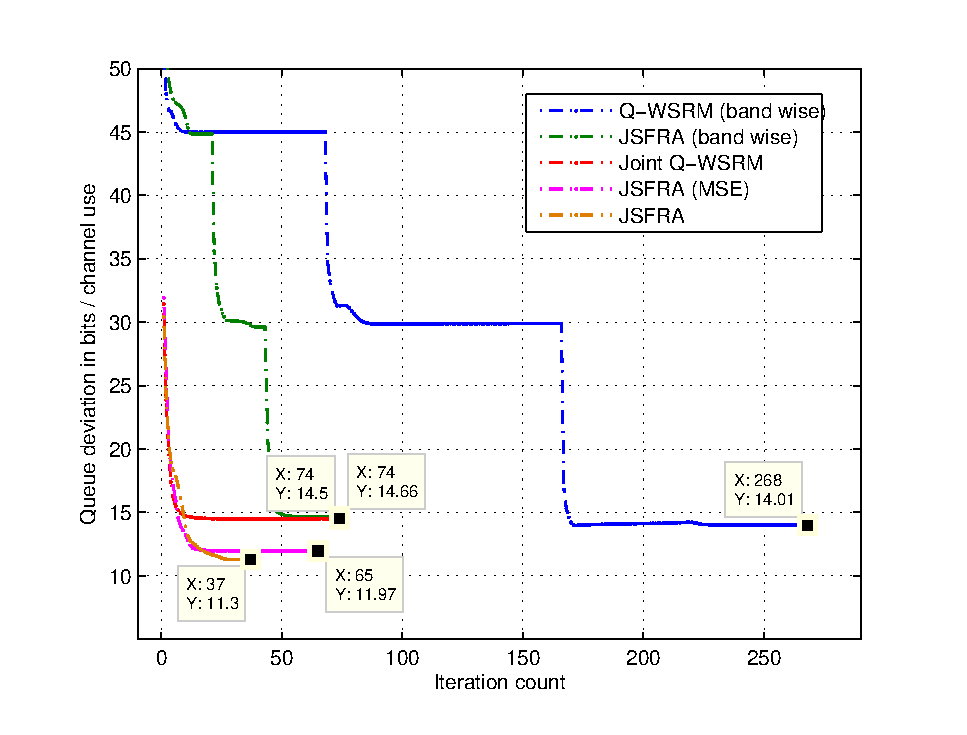
\includegraphics[width=1.0\textwidth]{fig-1}
\caption{\me{4 \times 1} system}
\label{fig-1}
\end{subfigure}
\hfill
\begin{subfigure}{0.49\textwidth}
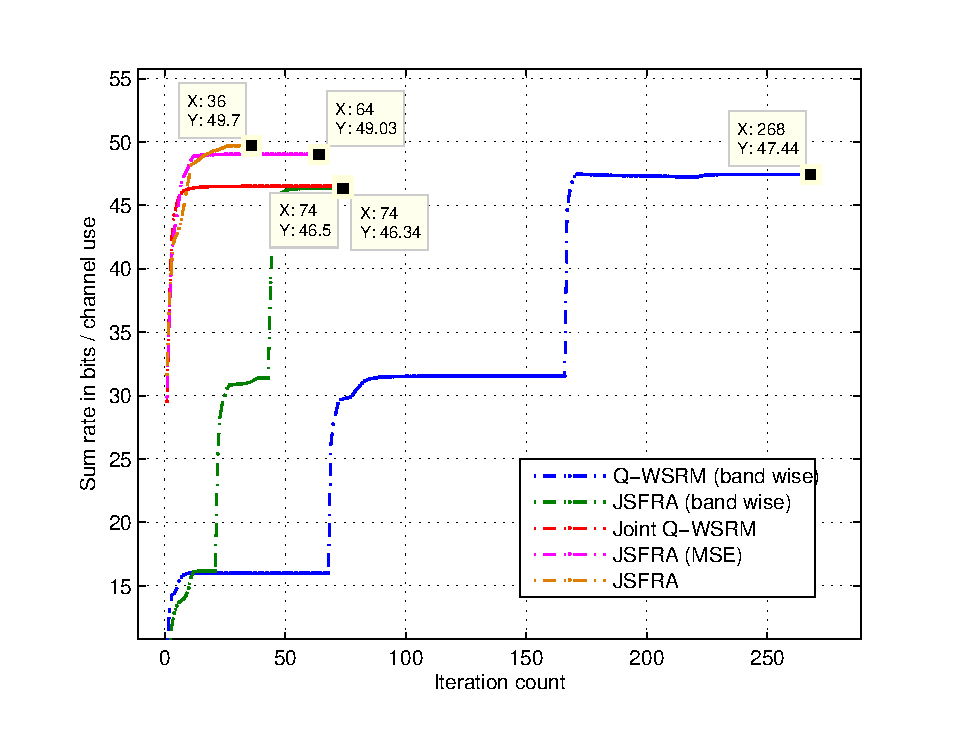
\includegraphics[width=1.0\textwidth]{fig-2}
\caption{\me{4 \times 2} system}
\label{fig-2}
\end{subfigure}
\caption{Convergence plot for \me{\lbrace N,N_B,K \rbrace = \lbrace 3,2,8 \rbrace} model}
\end{figure*}

Fig. \ref{fig-1} shows the performance of the above discussed schemes for a single receive antenna system. The figure compares the total number of \ac{SCA} iterations required by the \ac{JSFRA}, \ac{JSFRA} with sum power constraint, \ac{SRA} and \ac{Q-WSRM} schemes to achieve the optimal resource allocation to minimize the number of backlogged packets during the given scheduling instant. The convergence of the proposed \ac{JSFRA} is much quicker compared to the band-wise allocation schemes like the \ac{Q-WSRM} and the \ac{SRA} schemes. The waterfall like behavior for the band-wise allocation schemes suggests the rapid convergence when there is a band switch over, \textit{i.e}, when the queues are updated from the earlier sub-channels to find the precoders for the current sub-channel. The convergence at each sub-channel is iterated for the accuracy of \me{\approx 10^{-4}} or for a predetermined count \me{I_{\max}}, which creates the flat region between each waterfall behavior. The backlogged bits and the iteration count by various schemes at the convergence point are marked in the figures using data tips.
\begin{table}
\centering
\renewcommand{\arraystretch}{1.25} \scriptsize
\begin{tabular}{|c|*{8}{c}|c|}
\hline
\me{q} & \multicolumn{8}{c|}{user indices} & \me{\chi} \\
\hline
\me{1} & 12.0 &  4.22 &  5.51 & 9.21 &  8.04 & 12.0 & 12.0 & 9.84 & 23.18 \\
\me{2} & 9.65 & 7.67 & 8.57 & 8.79 & 8.63 & 9.13 & 9.54 & 9.08 & 24.94 \\
\me{\infty} & 8.71 & 8.71 & 8.71 & 8.71 & 8.71 & 8.71 & 8.71 & 8.71 & 26.34 \\
\hline
\end{tabular}
\caption{Queue information for \me{N=5} sub-channels}
\label{tbl-3}
\end{table}

Fig. \ref{fig-2} compares the convergence behavior of the precoder designs, which allocates the space-frequency resources to the users to minimize the number of backlogged packets. Different values for the exponent \me{q} are compared in Table \ref{tbl-3} for the system configuration \me{\{N_B,K,N_T,N_R\}= \{2,8,4,1\}}. The number of backlogged packets at each user before the current scheduling is fixed to be \me{12} bits. It is evident that the exponent \me{q=1} shows the greedy resource allocation in comparison with the fair scheduling achieved using \me{q=\infty}. The \me{q=\infty} norm does the fair scheduling even the path loss experienced by the users are different. It tries to minimize the variance across the backlogged packets of each user present in the system.

